\section{Stereo PIV Data processing}

Raw PIV data was processed into text files containing lists of vectors and 
positions from raw image data with commercial INSIGHT software. 
This format is considered to be the 
starting point for the present analysis. Each vector is recorded as a row in a 
"v3d" file, with a set of position coordinates,velocity 
vector components, and two quality control flags that were used to reduce 
spurious vector count. An example of this data is shown in Table 
\ref{table:v3d_row_example}.

\begin{table}[H]
\begin{center}
\begin{tabular}{|cccccccc|}
	\hline
	X mm & Y mm  & Z mm & U m/s & V m/s & W m/s & CHC & Residual Pixels\\
	\hline
	8.02046 & 0.174553 & 0 & 0.415872 & -2.25951 & 13.5873 & 1 & 0.127058\\
	9.74656 & 0.174553 & 0 & 0.386507 & -2.4523 & 13.9244 & 1 & 0.166965\\
	11.4727 & 0.174553 & 0 & 1.01919 & -2.8773 & 14.9454 & 1 & 0.0480147\\
	13.1988 & 0.174553 & 0 & 1.30872 & -3.02836 & 15.2081 & 1 & 0.0560525\\
	\hline
\end{tabular}
\caption{Example rows from v3d files with raw 3d vector data}
\label{table:v3d_row_example}
\end{center}
\end{table}


The position coordinates are expressed in units of millimeters from 
the fiducial mark on the target used for calibration. These coordinates are 
expressed from the viewpoint of the cameras, which were pointed upstream; 
positive $X$ coordinates are to the right, positive $Y$ is upwards, and 
positive $Z$ is towards the cameras. Vector components are recorded as $U$, 
$V$ and $W$. 

\subsection{Notation}
Since each run contained 200 separate vector sets, this data must be 
synthesized into 
values that compare well with the Reynolds Averaged Navier Stokes equations in 
cylindrical coordinates. This processing was performed in Python 2.7 and 
Matlab, with much of the code entirely replicated in each language. 
First, text files with tables of vector data were loaded into a parser to 
construct a mesh grid of the $X$, $Y$ coordinate space. These mesh grids 
establish the relationship between matrix indices and real coordinate 
space with units of $mm$.
Then, for each test as shown in Table \ref{table:test_matrix_table}, data from 
each of the 200 snapshots is Reynolds averaged to produce an average velocity 
component, and a fluctuating velocity component in each dimension for each 
vector, and expressed as equations \ref{eq:ubar} to \ref{eq:wprime}. 
Each component is given an individual variable name, with stable nonfluctuating 
components taken from an average of all sets expressed as capitol letters ($U$, 
$V$, $W$), and time averaged fluctuating components expressed as lower case 
letters ($u$, $v$, $w$). 
Velocities referring to just one of the 200 sets will use a 
subscript $i$ as ($U_i$, $V_i$, $W_i$). Each of these symbols represents an 
entire matrix of values across the interrogation plane. This is done primarily 
for simplicity and coherence between the theoretical basis, and the software 
implementation of 
the mathematics where special characters cannot be used in variable names.

\begin{equation}
U  = \frac{1}{N} \sum_{i=1}^{200} U_i
\label{eq:ubar}
\end{equation}

\begin{equation}
V  = \frac{1}{N} \sum_{i=1}^{200} V_i
\end{equation}

\begin{equation}
W  = \frac{1}{N} \sum_{i=1}^{200} W_i
\end{equation}

\begin{equation}
u = \frac{1}{N} \sum_{i=1}^{200} |U_i - U|
\end{equation}

\begin{equation}
v = \frac{1}{N} \sum_{i=1}^{200} |V_i - V|
\end{equation}

\begin{equation}
w = \frac{1}{N} \sum_{i=1}^{200} |W_i - W|
\label{eq:wprime}
\end{equation}

Where $U$, $V$ and $W$ are the time averaged velocity 
components in the $X$, $Y$, $Z$ directions respectively, and  $u$, 
$v$ and $w$ are the time averaged fluctuating velocity components.
Grid points with fewer than 20 measurements ($i < 20$) were assumed to be no 
data and thrown out. These fluctuating components can represent turbulent 
energies as $uu$, $vv$, and $ww$, and Reynolds stresses as $uv$, $vw$, and 
$uw$. Turbulent kinetic energy $k$ can be calculated as one half 
of the sum of the three components as in equation \ref{eq:tke}.

\begin{equation}
k = \frac{1}{2} \left(u^2 + v^2 + w^2\right)
\label{eq:tke}
\end{equation}


Once all the statistics for Cartesian coordinates have been generated, the 
vortex core must be found in order to convert all values to cylindrical 
coordinates. The core is found by finding the minimum in-plane velocity 
magnitudes near the center of the interrogation plane, excluding the stream 
wise $W$ component. In practice, to avoid confusion in identifying the vortex 
core due to spurious edge values, a threshold value is defined that limits the 
search for in-plane velocity minima to an area near the center of the field of 
view. Once the lowest value is found, sub-pixel accuracy is achieved by taking 
a cubic interpolation of the grid points surrounding the minimum, and resolving 
on the finer mesh grid. 

With a location for the vortex core, new mesh grids in radial and tangential 
coordinates, script $\mathcal{R}$ and $\theta$, are created from the $X$ and 
$Y$ mesh grids. velocity components in the $r$ and $t$ directions are then 
calculated by equations \ref{eq:uv_r} and \ref{eq:uv_t}.

\begin{equation}
R_i = u_i \cos{(\theta)} + v_i \sin{(\theta)}
\label{eq:uv_r}
\end{equation}

\begin{equation}
T_i = u_i \sin{(\theta)} - v_i \cos{(\theta)}
\label{eq:uv_t}
\end{equation}

Where $R_i$ and $T_i$ represent a radial and tangential velocity matrix for 
just one of the 200 total surveys, and $\theta$ is the mesh grid of angles 
about the vortex core. These equations are applied on an element wise basis to 
every $j,k$ grid point in the vector field. Once this is done, the same formula 
is applied to separate the radial and tangential velocity components $r$ and 
$t$ into stable and fluctuating components in equations \ref{eq:rbar} through 
\ref{eq:rbar}.

\begin{equation}
R  = \frac{1}{N} \sum_{i=1}^N R_i
\label{eq:rbar}
\end{equation}

\begin{equation}
T  = \frac{1}{N} \sum_{i=1}^N T_i
\label{eq:tbar}
\end{equation}

\begin{equation}
r = \frac{1}{N} \sum_{i=1}^N |R_i - R|
\end{equation}

\begin{equation}
t = \frac{1}{N} \sum_{i=1}^N |T_i - T|
\end{equation}

Where $R$ and $T$ are the time averaged velocity 
components in the $\mathcal{R}$ and $\theta$ directions respectively, and  $r$
and $t$ are the time averaged fluctuating velocity components.

Once this processing is complete, we have large set of reynolds averaged 
velocity data available for each of the 70 test cases. Plots of this data from 
test case 55 will be shown as examples. Stream plots can be produced as in 
figure \ref{fig:examp_stream}. Cartesian average velocity components for test 
case is shown in figures \ref{fig:examp_U} through \ref{fig:examp_W}, though 
they are not particularly useful when compared to values in cylindrical 
coordinates. 
Cylindrical average velocity components are shown in figures \ref{fig:examp_R} 
and \ref{fig:examp_T}. Reynolds stresses are shown in figures 
\ref{fig:examp_rt} through \ref{fig:examp_tw}. Turbulent energies are shown in 
figures \ref{fig:examp_rr} through \ref{fig:examp_ww}. Total turbulent kinetic 
energy $k$ is shown in figure \ref{fig:examp_tke}. Finally, scatter plots that 
flatten the dataset into one dimension can be generated as in the tangential 
velocity vs distance to core plot shown in figure \ref{fig:examp_Tscatter}.

\begin{figure}[H]
	\centering
	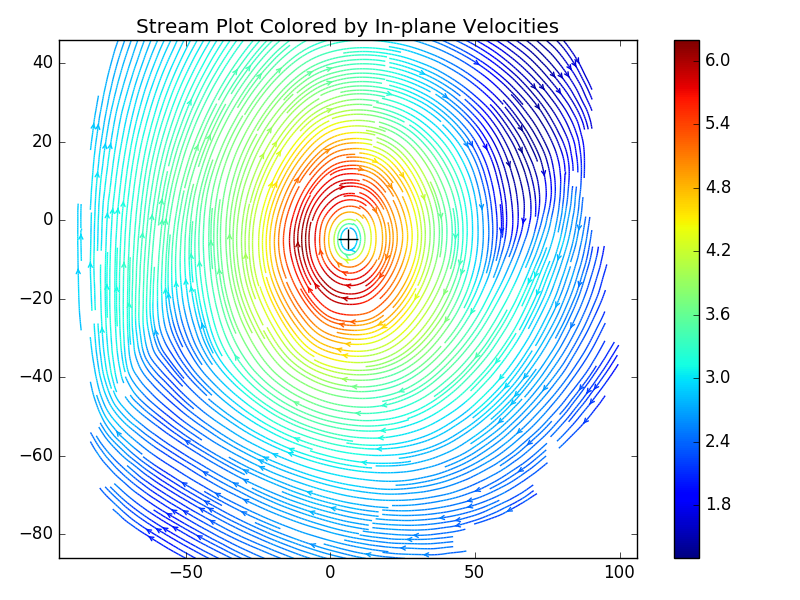
\includegraphics[width=5in]{figs/example_vortex_figs/example_stream}
	\caption{Example stream plot of run ID 55.}
	\label{fig:examp_stream}
\end{figure}

\begin{figure}[H]
	\centering
	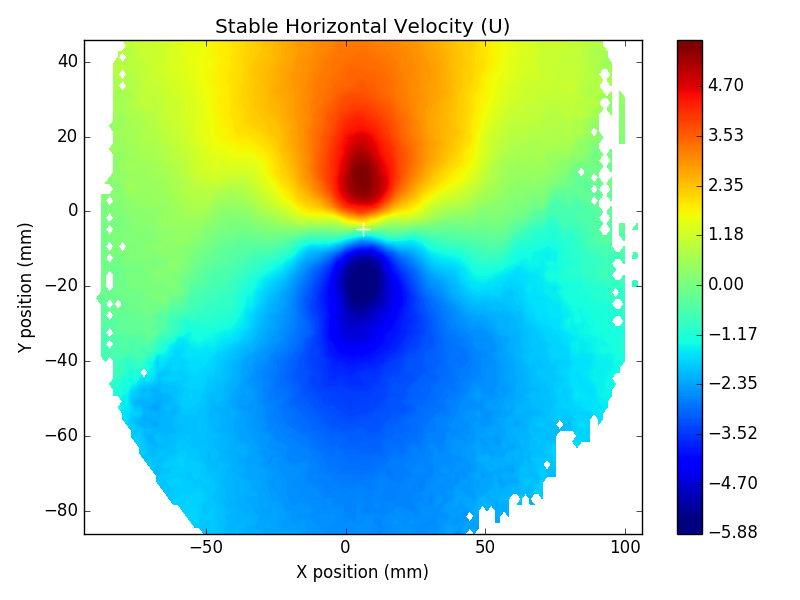
\includegraphics[width=5in]{figs/example_vortex_figs/example_U_contour}
\caption{Example contour plot of $U$ for run ID 55.}
\label{fig:examp_U}
\end{figure}

\begin{figure}[H]
	\centering
	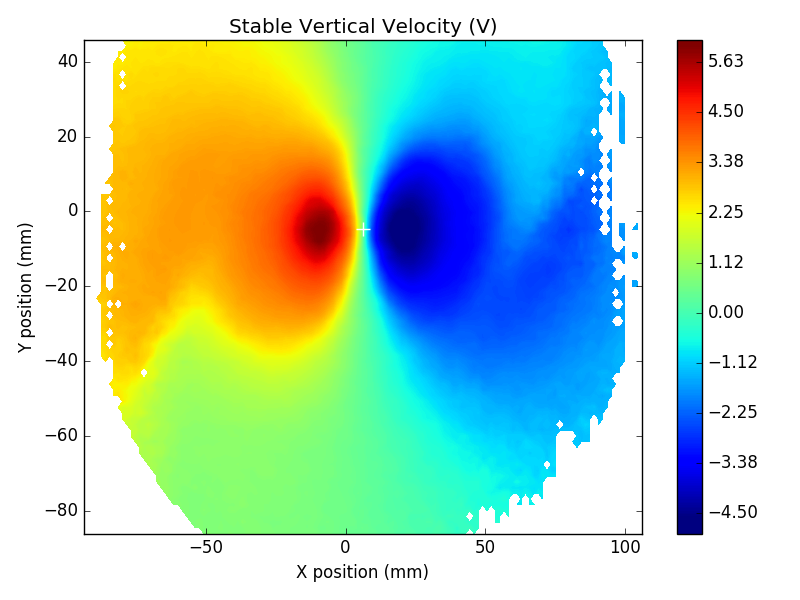
\includegraphics[width=5in]{figs/example_vortex_figs/example_V_contour}
\caption{Example contour plot of $V$ for run ID 55.}
\label{fig:examp_V}
\end{figure}

\begin{figure}[H]
	\centering
	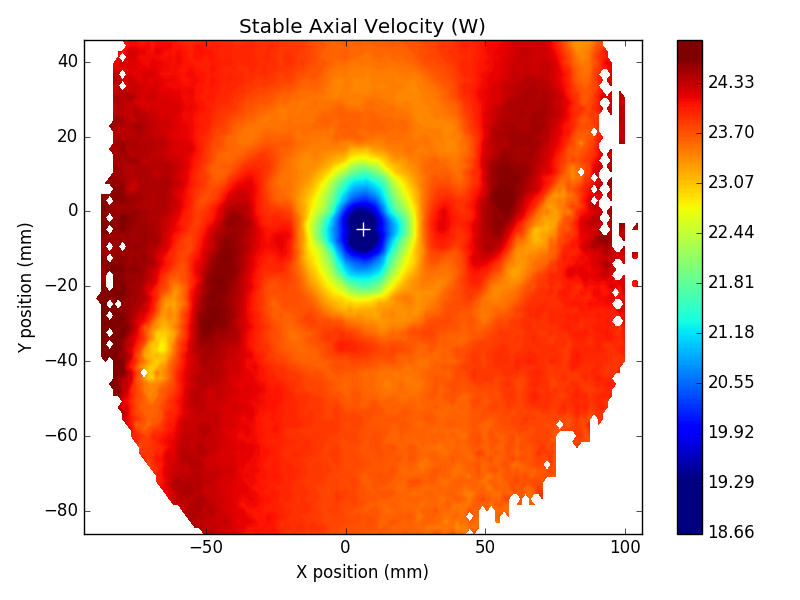
\includegraphics[width=5in]{figs/example_vortex_figs/example_W_contour}
\caption{Example contour plot of $W$ for run ID 55.}
\label{fig:examp_W}
\end{figure}

\begin{figure}[H]
	\centering
	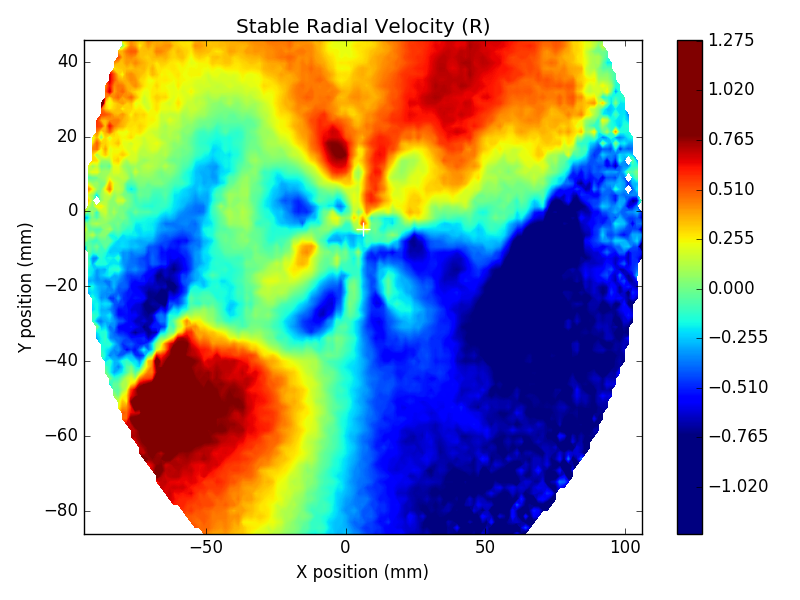
\includegraphics[width=5in]{figs/example_vortex_figs/example_R_contour}
\caption{Example contour plot of $R$ for run ID 55.}
\label{fig:examp_R}
\end{figure}

\begin{figure}[H]
	\centering
	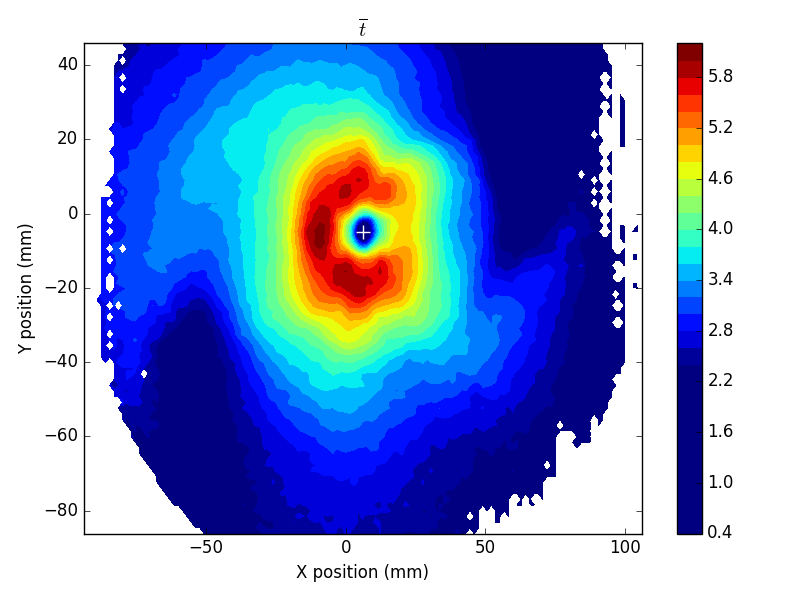
\includegraphics[width=5in]{figs/example_vortex_figs/example_T_contour}
\caption{Example contour plot of $T$ for run ID 55.}
\label{fig:examp_T}
\end{figure}

\begin{figure}[H]
	\centering
	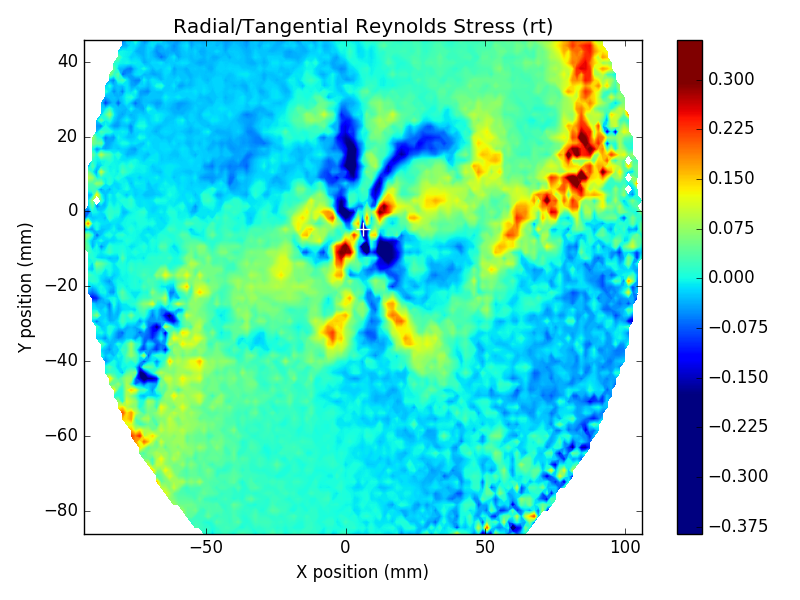
\includegraphics[width=5in]{figs/example_vortex_figs/example_rt_contour}
\caption{Example contour plot of $rt$ for run ID 55.}
\label{fig:examp_rt}
\end{figure}

\begin{figure}[H]
	\centering
	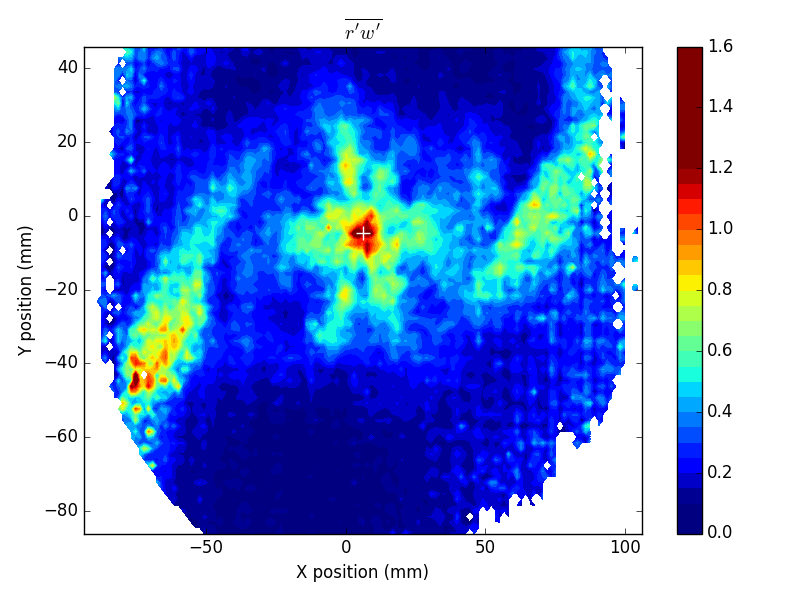
\includegraphics[width=5in]{figs/example_vortex_figs/example_rw_contour}
\caption{Example contour plot of $rw$ for run ID 55.}
\label{fig:examp_rw}
\end{figure}

\begin{figure}[H]
	\centering
	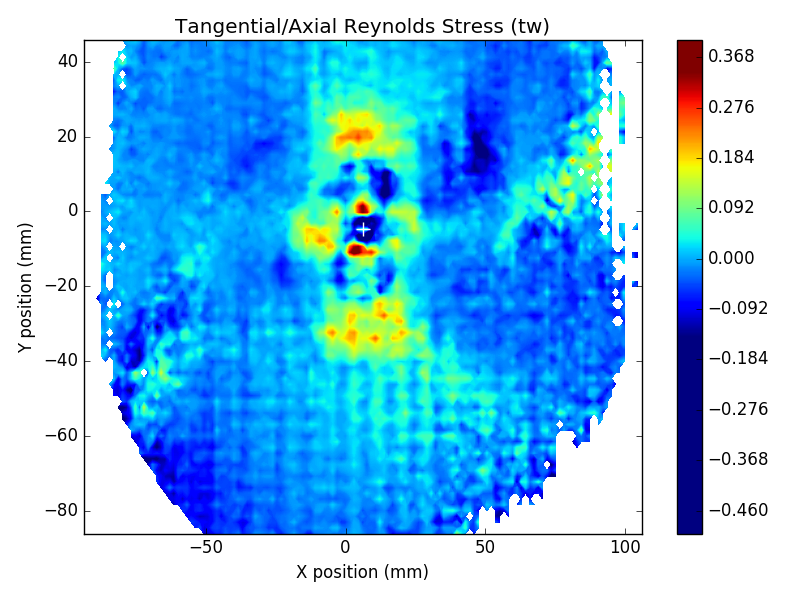
\includegraphics[width=5in]{figs/example_vortex_figs/example_tw_contour}
\caption{Example contour plot of $tw$ for run ID 55.}
\label{fig:examp_tw}
\end{figure}

\begin{figure}[H]
	\centering
	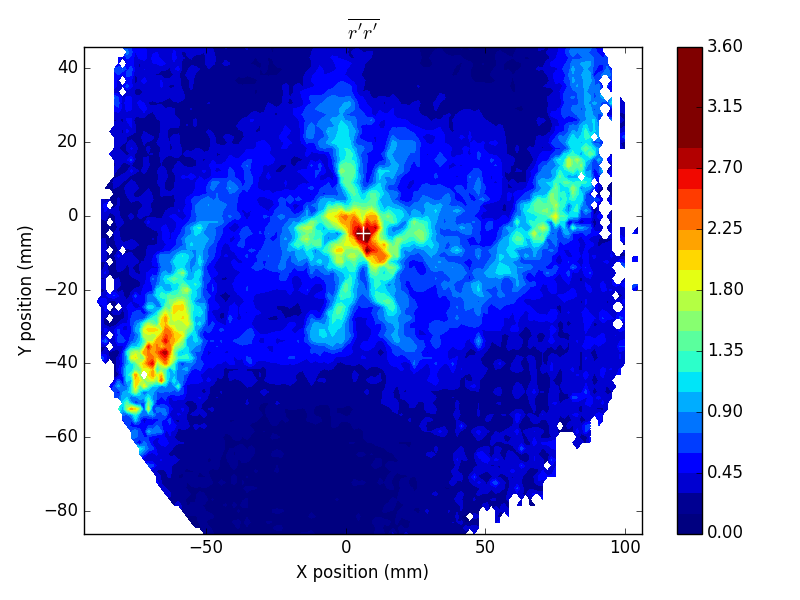
\includegraphics[width=5in]{figs/example_vortex_figs/example_rr_contour}
\caption{Example contour plot of $rr$ for run ID 55.}
\label{fig:examp_rr}
\end{figure}

\begin{figure}[H]
	\centering
	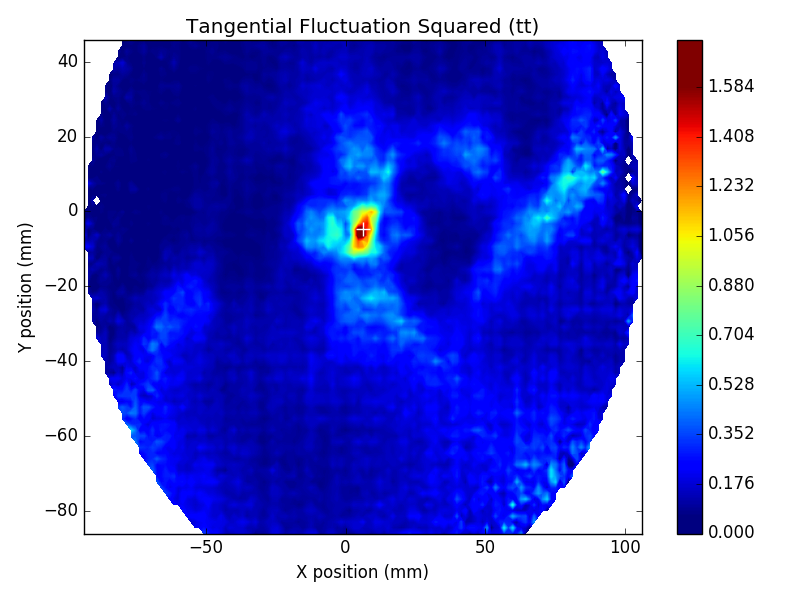
\includegraphics[width=5in]{figs/example_vortex_figs/example_tt_contour}
\caption{Example contour plot of $tt$ for run ID 55.}
\label{fig:examp_tt}
\end{figure}

\begin{figure}[H]
	\centering
	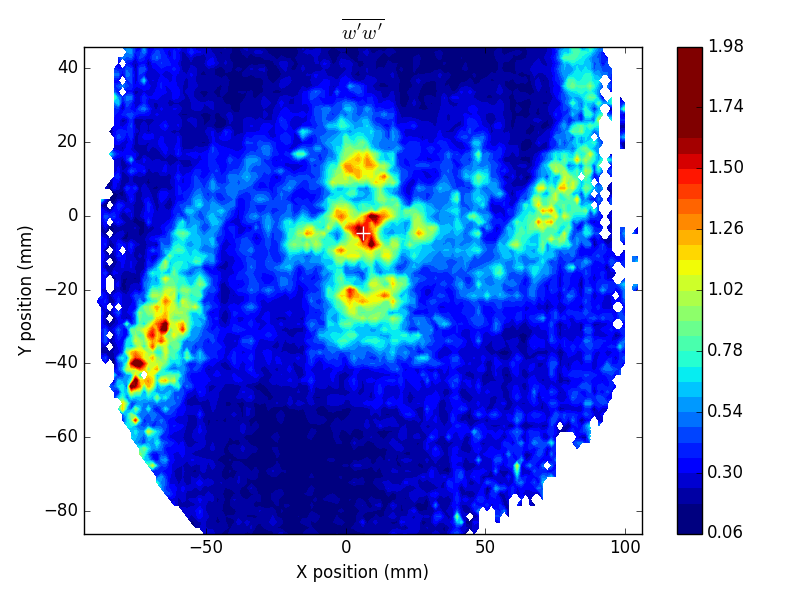
\includegraphics[width=5in]{figs/example_vortex_figs/example_ww_contour}
\caption{Example contour plot of $ww$ for run ID 55.}
\label{fig:examp_ww}
\end{figure}

\begin{figure}[H]
	\centering
	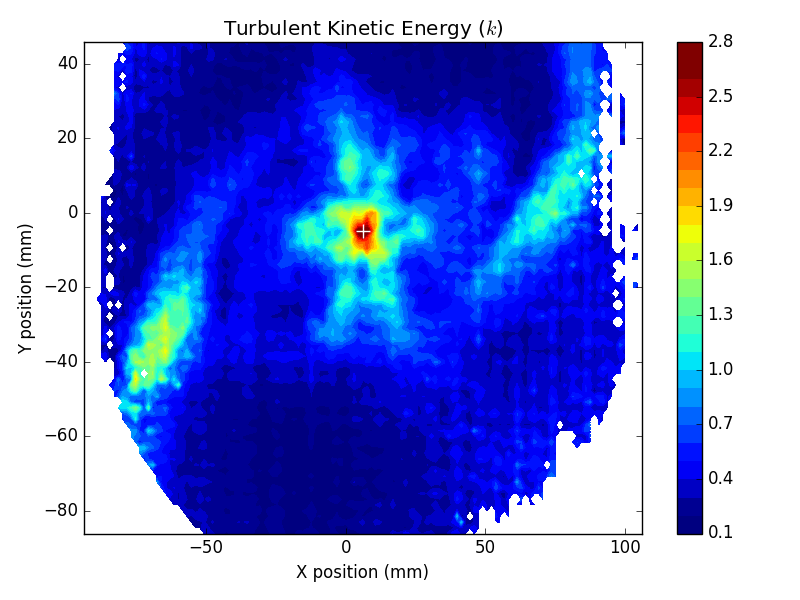
\includegraphics[width=5in]{figs/example_vortex_figs/example_ctke_contour}
\caption{Example contour plot of turbulent kinetic energy $k$ for run ID 55.}
\label{fig:examp_tke}
\end{figure}

\begin{figure}[H]
	\centering
	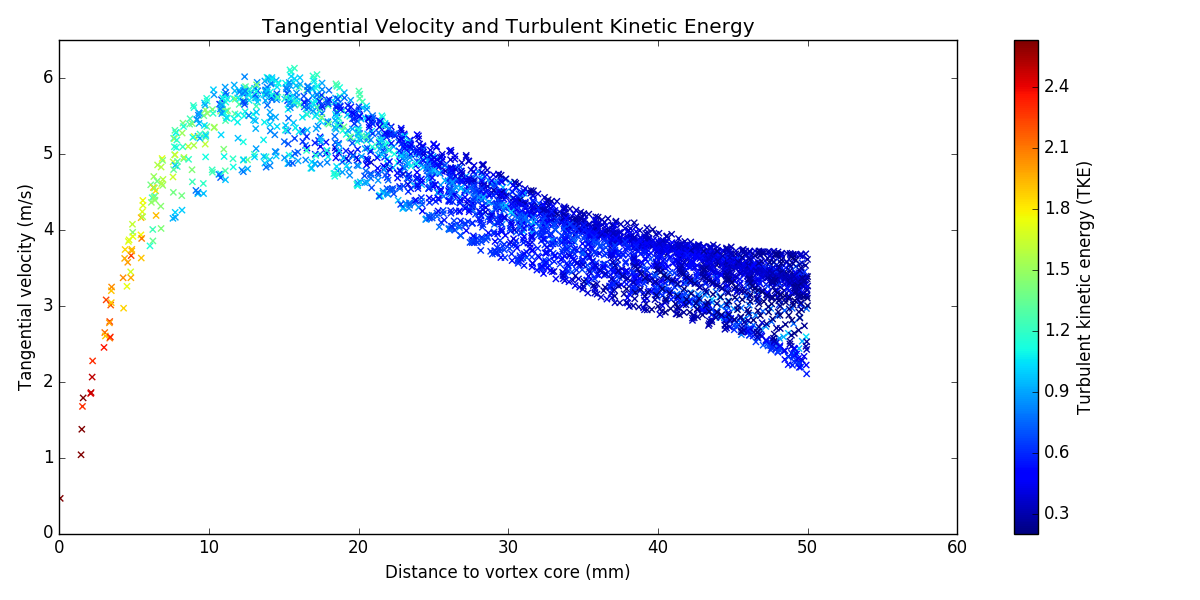
\includegraphics[width=7in]{figs/example_vortex_figs/example_TscatterTKE}
\caption{Example scatter plot of $T$, colored by $k$ for run ID 55.}
\label{fig:examp_Tscatter}
\end{figure}
